% THIS IS SIGPROC-SP.TEX - VERSION 3.0
% WORKS WITH V3.1SP OF ACM_PROC_ARTICLE-SP.CLS
% JUNE 2007
%
% It is an example file showing how to use the 'acm_proc_article-sp.cls' V3.1SP
% LaTeX2e document class file for Conference Proceedings submissions.
% ----------------------------------------------------------------------------------------------------------------
% This .tex file (and associated .cls V3.1SP) *DOES NOT* produce:
%       1) The Permission Statement
%       2) The Conference (location) Info information
%       3) The Copyright Line with ACM data
%       4) Page numbering
% ---------------------------------------------------------------------------------------------------------------
% It is an example which *does* use the .bib file (from which the .bbl file
% is produced).
% REMEMBER HOWEVER: After having produced the .bbl file,
% and prior to final submission,
% you need to 'insert'  your .bbl file into your source .tex file so as to provide
% ONE 'self-contained' source file.
%
% Questions regarding SIGS should be sent to
% Adrienne Griscti ---> griscti@acm.org
%
% Questions/suggestions regarding the guidelines, .tex and .cls files, etc. to
% Gerald Murray ---> murray@acm.org
%
% For tracking purposes - this is V3.0SP - JUNE 2007

% \documentclass{acm_proc_article-sp}
\documentclass{sig-alternate}

\graphicspath{{figures/}}

\begin{document}

\title{Software Trajectory Analysis:\\An empirically based method for automated software process discovery}

%\numberofauthors{8} %  in this sample file, there are a *total*
% of EIGHT authors. SIX appear on the 'first-page' (for formatting
% reasons) and the remaining two appear in the \additionalauthors section.
%
\numberofauthors{1}
\author{
% You can go ahead and credit any number of authors here,
% e.g. one 'row of three' or two rows (consisting of one row of three
% and a second row of one, two or three).
%
% The command \alignauthor (no curly braces needed) should
% precede each author name, affiliation/snail-mail address and
% e-mail address. Additionally, tag each line of
% affiliation/address with \affaddr, and tag the
% e-mail address with \email.
%
% 1st. author
\alignauthor Pavel Senin \\
\affaddr{Collaborative Software Development Laboratory}\\
\affaddr{University of Hawaii at Manoa}\\
\affaddr{POST 307, 1680 East-West Rd.}\\
\affaddr{Honolulu, HI 96822}\\
\email{senin@hawaii.edu}
}
% There's nothing stopping you putting the seventh, eighth, etc.
% author on the opening page (as the 'third row') but we ask,
% for aesthetic reasons that you place these 'additional authors'
% in the \additional authors block, viz.
%\additionalauthors{Additional authors: John Smith (The Th{\o}rv{\"a}ld Group,
%email: {\texttt{jsmith@affiliation.org}}) and Julius P.~Kumquat
%(The Kumquat Consortium, email: {\texttt{jpkumquat@consortium.net}}).}
%\date{30 July 1999}
% Just remember to make sure that the TOTAL number of authors
% is the number that will appear on the first page PLUS the
% number that will appear in the \additionalauthors section.

\maketitle
\begin{abstract}
For structuring and planning of effort in software development software processes were modeled with an expert intuition and apriori knowledge for the long time resulting in Waterfal, Spiral and other models. Later, with a wide use of SCM systems and public availability of software process artifact trails, formal methods such as Petri Nets, FSM and others were applied for recurrent processes discovery and control. With increase in use of in-process software engineering measurement and analysis software systems new types of software process artifacts becoming available. In this work I propose to investigate an automated technique for the discovery and characterization of recurrent behaviors in software development - ``programming habits'' either on an individual or a team level.
\end{abstract}

% A category with the (minimum) three required fields
%\category{H.4}{Information Systems Applications}{Miscellaneous}
%A category including the fourth, optional field follows...
%\category{D.2.8}{Software Engineering}{Metrics}[complexity measures, performance measures]

%\terms{Software process}

%\keywords{ACM proceedings, \LaTeX, text tagging} % NOT required for Proceedings

\section{Introduction and Motivation}
A \textit{software process} is a set of activities performed in order to design, develop and maintain software systems. Examples of such activities include design methods; requirements collection and creation of UML diagrams; testing and performance analysis. The primary intent behind a software process is to structure and coordinate human activities in order to achieve the goal - deliver a software system successfully; the secondary intent would be to design a set and asequence of processes which reproduce such a success as well as to be able to improve the process performance.

Much work has been done in software process research resulting in a number of industrial standards for process models (CMM, ISO, PSP etc. \cite{citeulike:5043104}) which are widely accepted by many goverment and industrial institutions. Nevertheless, software development remains error-prone and more than a half of all software development projects ending up failing or being very poorly executed. Some of them are abandoned due to running over budget, some are delivered with such low quality or so late that they are useless, and some, when delivered, are never used because they do not fulfill requirements \cite{citeulike:7351135}. The cost of this lost effort is enormous and may in part be due to our incomplete understanding of software process.

There is a long history of software process improvement through proposing specific patterns of software development. For example, the Waterfall Model process proposes a sequential pattern in which developers first create a Requirements document, then create a Design, then create an Implementation, and finally develop Tests. The Test Driven Development process proposes an iterative pattern in which the developer must first write a test case, then write the code to implement that test case, then refactor the system for maximum clarity and minimal code duplication. Probably the main problem with the traditional top-down approach to process development is that it requires the developer or manager to notice a recurrent pattern of behavior in the first place \cite{citeulike:5043104}. 

A an alternative to that, in my research, I am applying knowledge discovery and data mining techniques to the domain of software engineering in order to evaluate their ability to automatically notice interesting recurrent patterns of behavior from collected software process artifacts. While I am not proposing to be able to infer a complete and correct software process model, my system will provide its users with a formal description of recurrent behaviors in their software development. As a simple example, consider a development team in which committing code to a repository triggers a build of the system. Sometimes the build passes, and sometimes the build fails. To improve the productivity of the team, it would be useful to be aware of any recurrent behaviors of the developers. My system might generate one recurrent pattern consisting of a) implementing code b) running unit tests, c) committing code and d) a passed build: $i \rightarrow u \rightarrow c \rightarrow s $, and another recurrent pattern consisting of a) implementing code, b) committing code, and c) a failed build: $i \rightarrow c \rightarrow f $. The automated generation of these recurrent patterns can provide actionable knowledge to developers; in this case, the insight that running test cases prior to committing code reduces the frequency of build failures.

Although the latest trends in software process research emphasize mining of software process artifacts and behaviors \cite{citeulike:5043664} \cite{citeulike:1885717} \cite{citeulike:5112229} \cite{citeulike:1885717}, to the best of my knowledge, the approach I am taking has never been attempted. This may be partly due to the lack of means of automated, real-time data collection of fine-grained developer behaviors. By leveraging the ability of the Hackystat system \cite{citeulike:4041809} to collect such a fine grained data, I propose to extend previous research with new knowledge that will support improvements in our understanding of software process.

\section{Relevant prior work}
Even though process mining in the business domain is a well-established field with much software developed up to date (ERP, WFM and other systems), ``Business Process Intelligence'' tools usually do not perform process discovery and typically offer relatively simple analyses that depend upon a correct a-priori process model \cite{citeulike:3718014} \cite{citeulike:5044991}. This fact restricts direct application of business domain process mining techniques to software engineering, where processes are usually performed concurrently by many agents, are more complex and typically have a higher level of noise. Taking this fact in account, I will review only the approaches to the mining for which applicability to software process mining was expressed. 

Perhaps, the research most relevant to my own was done by Cook \& Wolf in \cite{citeulike:328044}. The authors developed a \textit{``process discovery''} techniques intended to discover process models from event streams. The authors did not really intend to generate a complete model, but rather to generate sub-models that express the most frequent patterns in the event stream. They designed a framework which collects process data from ongoing software process or from history logs, and generates a set of recurring patterns of behavior characterizing observed process. In this work they extended two methods of \textit{grammar inference} from previous work: purely statistical (neural network based \textit{RNet}) and purely algorithmic (\textit{KTail}) as well as developing their own Markovian method (\textit{Markov}). 

Process discovery, in the author's opinion, resembles the process of grammar inference, which can be defined as a process of inferring a language grammar from the given set (sample) of sentences in this language. In the demonstrated approach, words of the language are atomic events of the dynamic process, whether sentences built from such words, are describing the behavior of a process. Consequently, the inferred grammar of that language is the formal model of the process. Cook \& Wolf expressed such grammars as Finite State Machines (FSMs) and implemented a software tool for the mining of the software process. This tool was successfully tested in an industrial case study.

\begin{figure}[tbp]
   \centering
   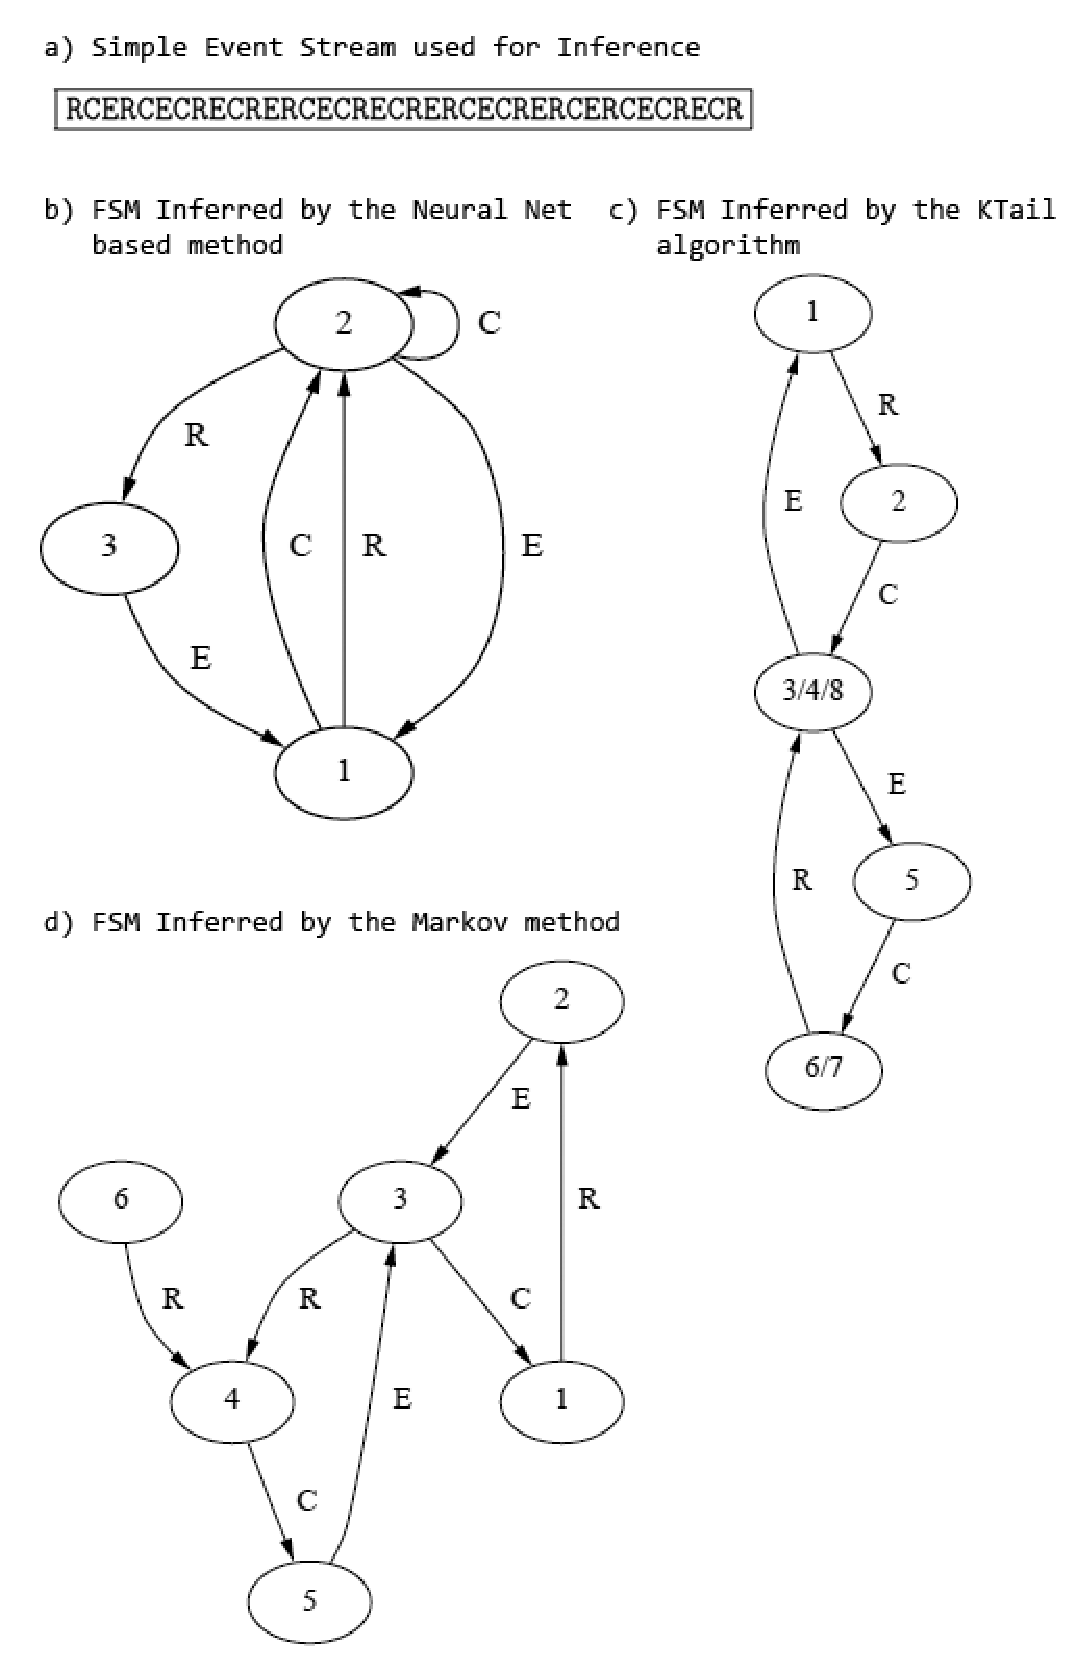
\includegraphics[height=45mm]{inference.eps}
   \caption{Process discovery through the grammar inference: panel a) a sample event stream (simple process involving three types of events: Edit, Review, and Checkin); and FNA results obtained by applying three methods of process discovery from Cook \& Wolf \cite{citeulike:328044}.}
   \label{fig:inference}
\end{figure}

The first method extended by the authors, the neural-network based grammar inference, RNet algorithm, defines a recurrent neural network architecture which is trained by the sequences of events. After training, this neural net is able to characterize a current system state by looking on past behavior. The authors extract the FSM from the trained neural network by presenting different strings to it and extracting the hidden neurons activity through observations. Due to the nature of Neural Net, closely related activation patterns are clustered into the same state; therefore, by noting the current pattern, the input token, and the next activation pattern, transitions are recorded and compiled into the inferred FSM.

The second method investigated, is a purely algorithmic KTail method, which was taken from the work of Biermann \& Feldman \cite{citeulike:5120603}. The idea is that a current state is defined by what future behaviors can occur from it. The \textit{future} is defined as the set of next $k$ tokens. By looking at a window of successor events, the KTail algorithm can build the equivalence classes that compose the process model. The authors extensively modified the original KTail algorithm improving the folding in the mined model making it more robust to noise.

The Markov based method developed by the authors is based on both algorithmic and statistical approaches. It takes to account past and future system behavior in order to guess the current system state. Assuming that a finite number of states can define the process, and that the probability of the next state is based only on the current state (Markov property), the authors built a $n^{th}$-order Markov model using the first and second order probabilities. Once built, the transition probability table corresponding to the Markov model is converted into FSM which is in turn reduced based on the user-specified cut-off threshold for probabilities.

The authors implemented all three of these algorithms in a software tool called \textsc{DaGama} as a plugin for larger software system called Balboa \cite{citeulike:5120757}. By performing benchmarking, Cook \& Wolf found that the Markov algorithm was superior to the two others. RNet was found to be the worst of the three algorithms. 

Overall, while having some issues with the complexity of produced output and noise handling, the authors proved applicability of implemented algorithms to real-world process data by demonstrating an abstraction of the actual process executions and capturing important properties of the process behavior. The major backdraw of the approach, as stated by the authors, lies in the inability of the FSMs to model concurrency of processes which limits its applicability to the software development process. Later, Cook et al. in \cite{citeulike:5128143} addressed this limitation by using Petri-nets and Moore-type FSM.

Another set of findings relevant to my research approach was developed by Rubin et al. \cite{citeulike:1885717} and van der Aalst et al. \cite{citeulike:3718014} and is called \textit{incremental workflow mining}. The authors not only designed sophisticated algorithms but built a software system using a business process mining framework called ProM by van Dongen et al. \cite{citeulike:5043673} which synthesizes a Petri Net corresponding to the observed process. The system was tested on SCM logs and while the process artifacts retrieved from the SCM system are rather high-level, the approach discussed is very promising for the modeling of software processes from the low-level product and process data.

\begin{figure}[tbp]
   \centering
   \includegraphics[height=35mm]{petri.eps}
   \caption{Illustration of the ``Generation and Synthesis Approach'' from \cite{citeulike:5043673}: a) Transition System with regions shown; b),c) Petri Nets synthesized from the Transition System.}
   \label{fig:petri}
\end{figure}

Within the incremental workflow mining framework, the input data from the SCM audit trail information is mapped to the event chain which corresponds to the software process artifacts. The authors call this process \textit{abstraction on the log level} which is implemented as a set of filters which not only aggregates basic events into single high-level entities but also removes data irrelevant to the mining process (noise). 

The event chain constructed through the abstraction is then treated with the \textit{Generate} part of the \textit{``Generate and Synthesis''} \cite{citeulike:3718014} algorithm in order to generate a \textit{Transition System} which represents an ordered series of events. This algorithm looks at the history (prefix) and the future (suffix) sequences of events related to the current one in order to discover transitions.  When applied to the abstracted log information, the algorithm generates a rather large Transition System graph where edges connect to abstracted events. This transition system is then successively simplified by using various reduction strategies. At the last step of the incremental workflow mining approach, Transition Systems are used to \textit{Synthesize} labeled Petri nets (where different transition can refer to the same event) with the help of \textit{``regions theory''} \cite{citeulike:5128170}. As with the Transition System generation, the authors investigate many different strategies of Petri nets synthesis, showing significant variability in the results achieved. (see Figure \ref{fig:petri}).

The significant contribution of this research is in the generality of the method. It was shown that by tuning the ``Generate'' and ``Synthesize'' phases it is possible to tailor the algorithm to a wide variety of processes. In particular, as mentioned before, Rubin et al. successfully applied this framework to the SCM logs analysis.

\section{Research objectives}
As shown by previous research, it is possible to infer and successively formalize software process by observing its artifacts, and in particular, recurrent behavioral patterns. The problem of finding such patterns is the cornerstone of my research. My approach to this problem rests on the application of data-mining techniques to symbolic time-point and time-interval series constructed directly from the real-valued telemetry streams provided by Hackystat.

\begin{figure}[tbp]
   \centering
   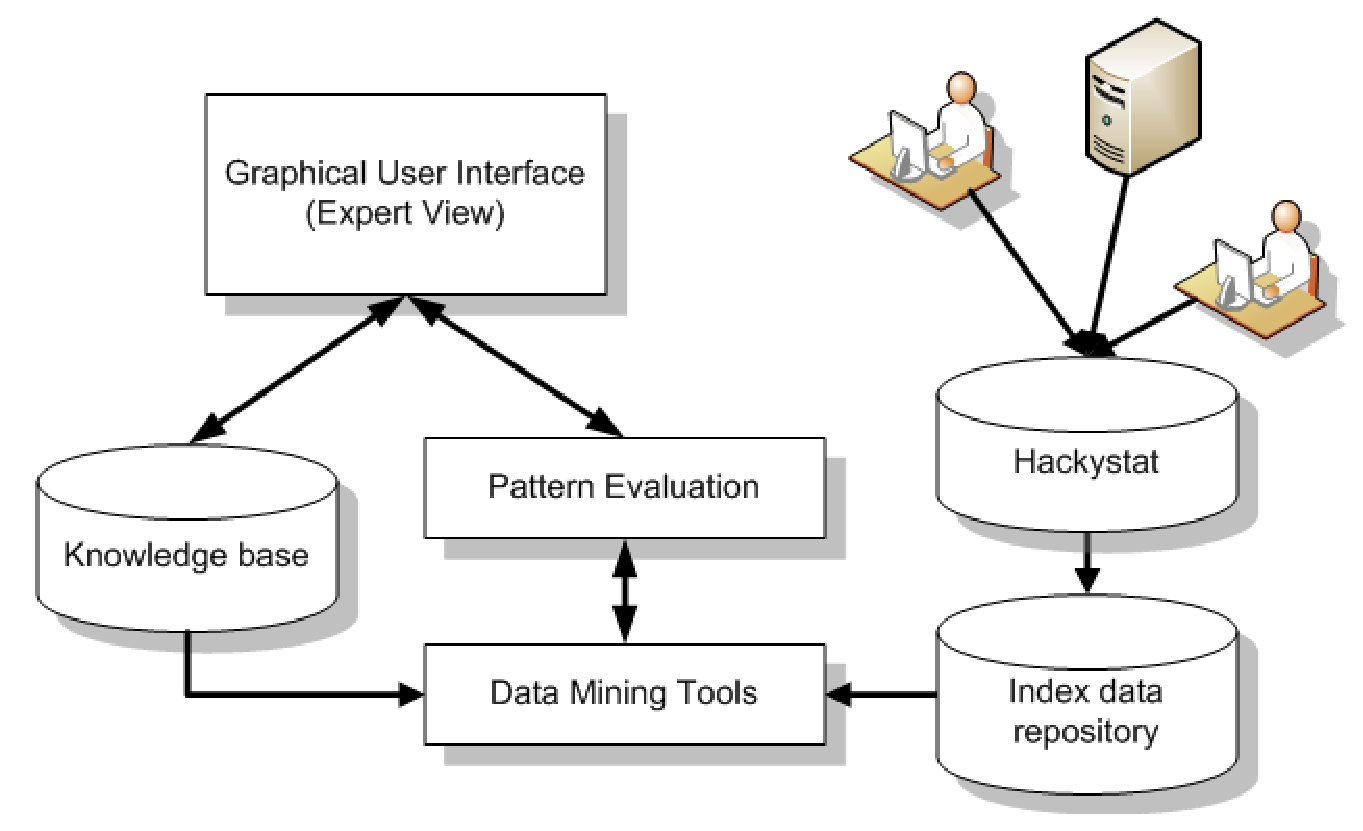
\includegraphics[height=50mm]{system_overview.eps}
   \caption{The high-level system overview. Software engineering process and product data are collected and aggregated by Hackystat and then used to generate temporal symbolic indexes. Data mining tools constrained by software engineering domain knowledge are then used for unsupervised patterns discovery. The GUI provides an interface to the discovered patterns and aids in investigation of a discovered phenomena.}
   \label{fig:system_overview}
\end{figure}

To investigate the requirements for a software tool that aids in the discovery of recurrent behavioral patterns in software process, I am designing and developing the ``Software Trajectory'' framework. A high-level overview of the framework is shown in Figure \ref{fig:system_overview} and resembles the flow of the ``Knowledge Discovery in Database'' process discussed by Han et al. in \cite{citeulike:709476}. As shown, the data collected by Hackystat is transformed into a symbolic format and then indexed for further use in data-mining. The tools, designed for data-mining, have a specific restrictions placed on the search space by domain and context knowledge in an attempt to limit the amount of reported patterns to useful ones. I am planning to design a GUI in a way that will allow easy access and modification of these restrictions. 


\section{Research approach}

\section{Data analysis methods}

\section{Empirical study design}

\section{Conclusions}
This paragraph will end the body of this sample document.
Remember that you might still have Acknowledgments or
Appendices; brief samples of these
follow.  There is still the Bibliography to deal with; and
we will make a disclaimer about that here: with the exception
of the reference to the \LaTeX\ book, the citations in
this paper are to articles which have nothing to
do with the present subject and are used as
examples only.
%\end{document}  % This is where a 'short' article might terminate

%ACKNOWLEDGMENTS are optional
\section{Acknowledgments}
This section is optional; it is a location for you
to acknowledge grants, funding, editing assistance and
what have you.  In the present case, for example, the
authors would like to thank Gerald Murray of ACM for
his help in codifying this \textit{Author's Guide}
and the \textbf{.cls} and \textbf{.tex} files that it describes.

%
% The following two commands are all you need in the
% initial runs of your .tex file to
% produce the bibliography for the citations in your paper.
\bibliographystyle{abbrv}
\bibliography{seninp}  % sigproc.bib is the name of the Bibliography in this case
% You must have a proper ".bib" file
%  and remember to run:
% latex bibtex latex latex
% to resolve all references
%
% ACM needs 'a single self-contained file'!
%
%APPENDICES are optional
%\balancecolumns
\appendix
%Appendix A
\section{Headings in Appendices}
The rules about hierarchical headings discussed above for
the body of the article are different in the appendices.
In the \textbf{appendix} environment, the command
\textbf{section} is used to
indicate the start of each Appendix, with alphabetic order
designation (i.e. the first is A, the second B, etc.) and
a title (if you include one).  So, if you need
hierarchical structure
\textit{within} an Appendix, start with \textbf{subsection} as the
highest level. Here is an outline of the body of this
document in Appendix-appropriate form:
\subsection{Introduction}
\subsection{The Body of the Paper}
\subsubsection{Type Changes and  Special Characters}
\subsubsection{Math Equations}
\paragraph{Inline (In-text) Equations}
\paragraph{Display Equations}
\subsubsection{Citations}
\subsubsection{Tables}
\subsubsection{Figures}
\subsubsection{Theorem-like Constructs}
\subsubsection*{A Caveat for the \TeX\ Expert}
\subsection{Conclusions}
\subsection{Acknowledgments}
\subsection{Additional Authors}
This section is inserted by \LaTeX; you do not insert it.
You just add the names and information in the
\texttt{{\char'134}additionalauthors} command at the start
of the document.
\subsection{References}
Generated by bibtex from your ~.bib file.  Run latex,
then bibtex, then latex twice (to resolve references)
to create the ~.bbl file.  Insert that ~.bbl file into
the .tex source file and comment out
the command \texttt{{\char'134}thebibliography}.
% This next section command marks the start of
% Appendix B, and does not continue the present hierarchy
\section{More Help for the Hardy}
The acm\_proc\_article-sp document class file itself is chock-full of succinct
and helpful comments.  If you consider yourself a moderately
experienced to expert user of \LaTeX, you may find reading
it useful but please remember not to change it.
\balancecolumns
% That's all folks!
\end{document}
